\indent En esta secci\'on, mostraremos buenos y malos casos para nuestro algoritmo, y a su vez, daremos el tiempo estimado 
seg\'un la complejidad del algoritmo calculada anteriormente.

Como la complejidad presenta dos variables marcadas, como son las capacidades de las mochilas y la cantidad de objetos, hemos trabajado con las mismas en simultaneo y tambi\'en fijando alguna de las dos variables.\\


Chequeando la familia de casos que enunciamos en el anterior inciso pudimos llegar a la conclusion que teniendo capacidades identicas en las mochilas o distintas nuestro algoritmo se comporta a nivel tiempo de ejecuci\'on de una manera similar, por lo tanto trabajaremos a continuaci\'on con capacidades distintas.\\

A continuaci\'on mostraremos dos graficos que simbolizan el tiempo de ejecuci\'on de cada una de las familias de casos:\\

\vspace*{0.3cm} \vspace*{0.3cm}
  \begin{center}
 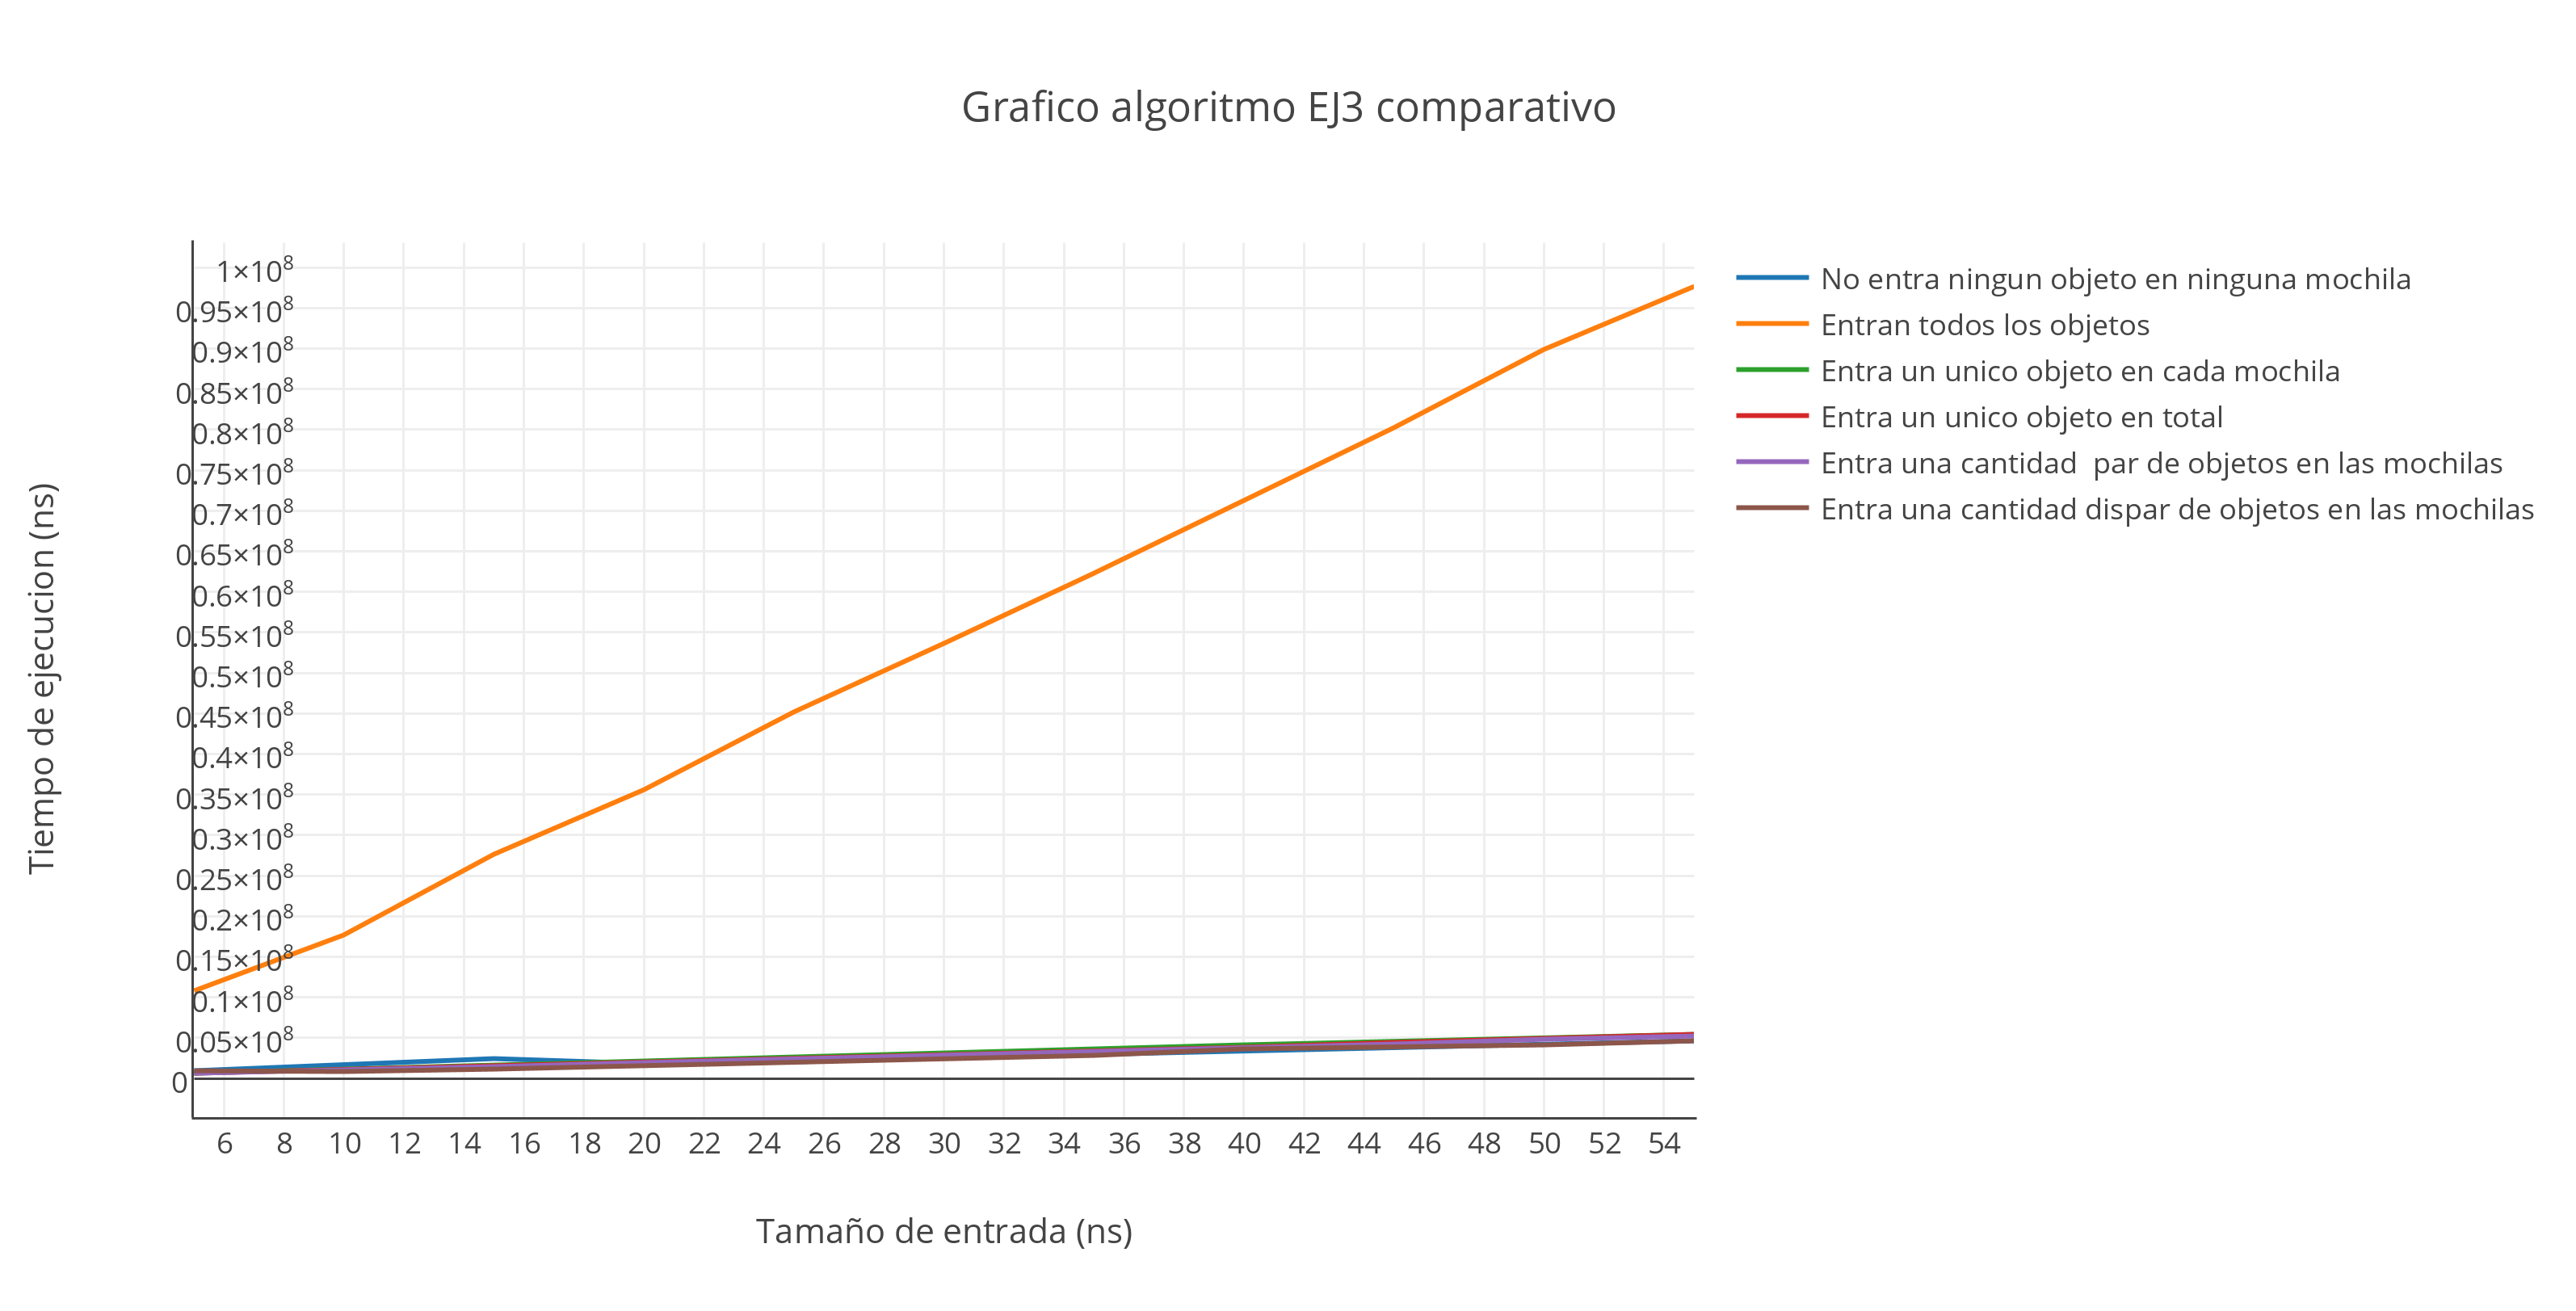
\includegraphics[scale=0.65]{./EJ3/comparativo.png}
 {$Gr$\'a$fico$ \ 3.1 - $Comparativo$}
  \end{center}
  \vspace*{0.3cm}

\vspace*{0.3cm} \vspace*{0.3cm}
  \begin{center}
 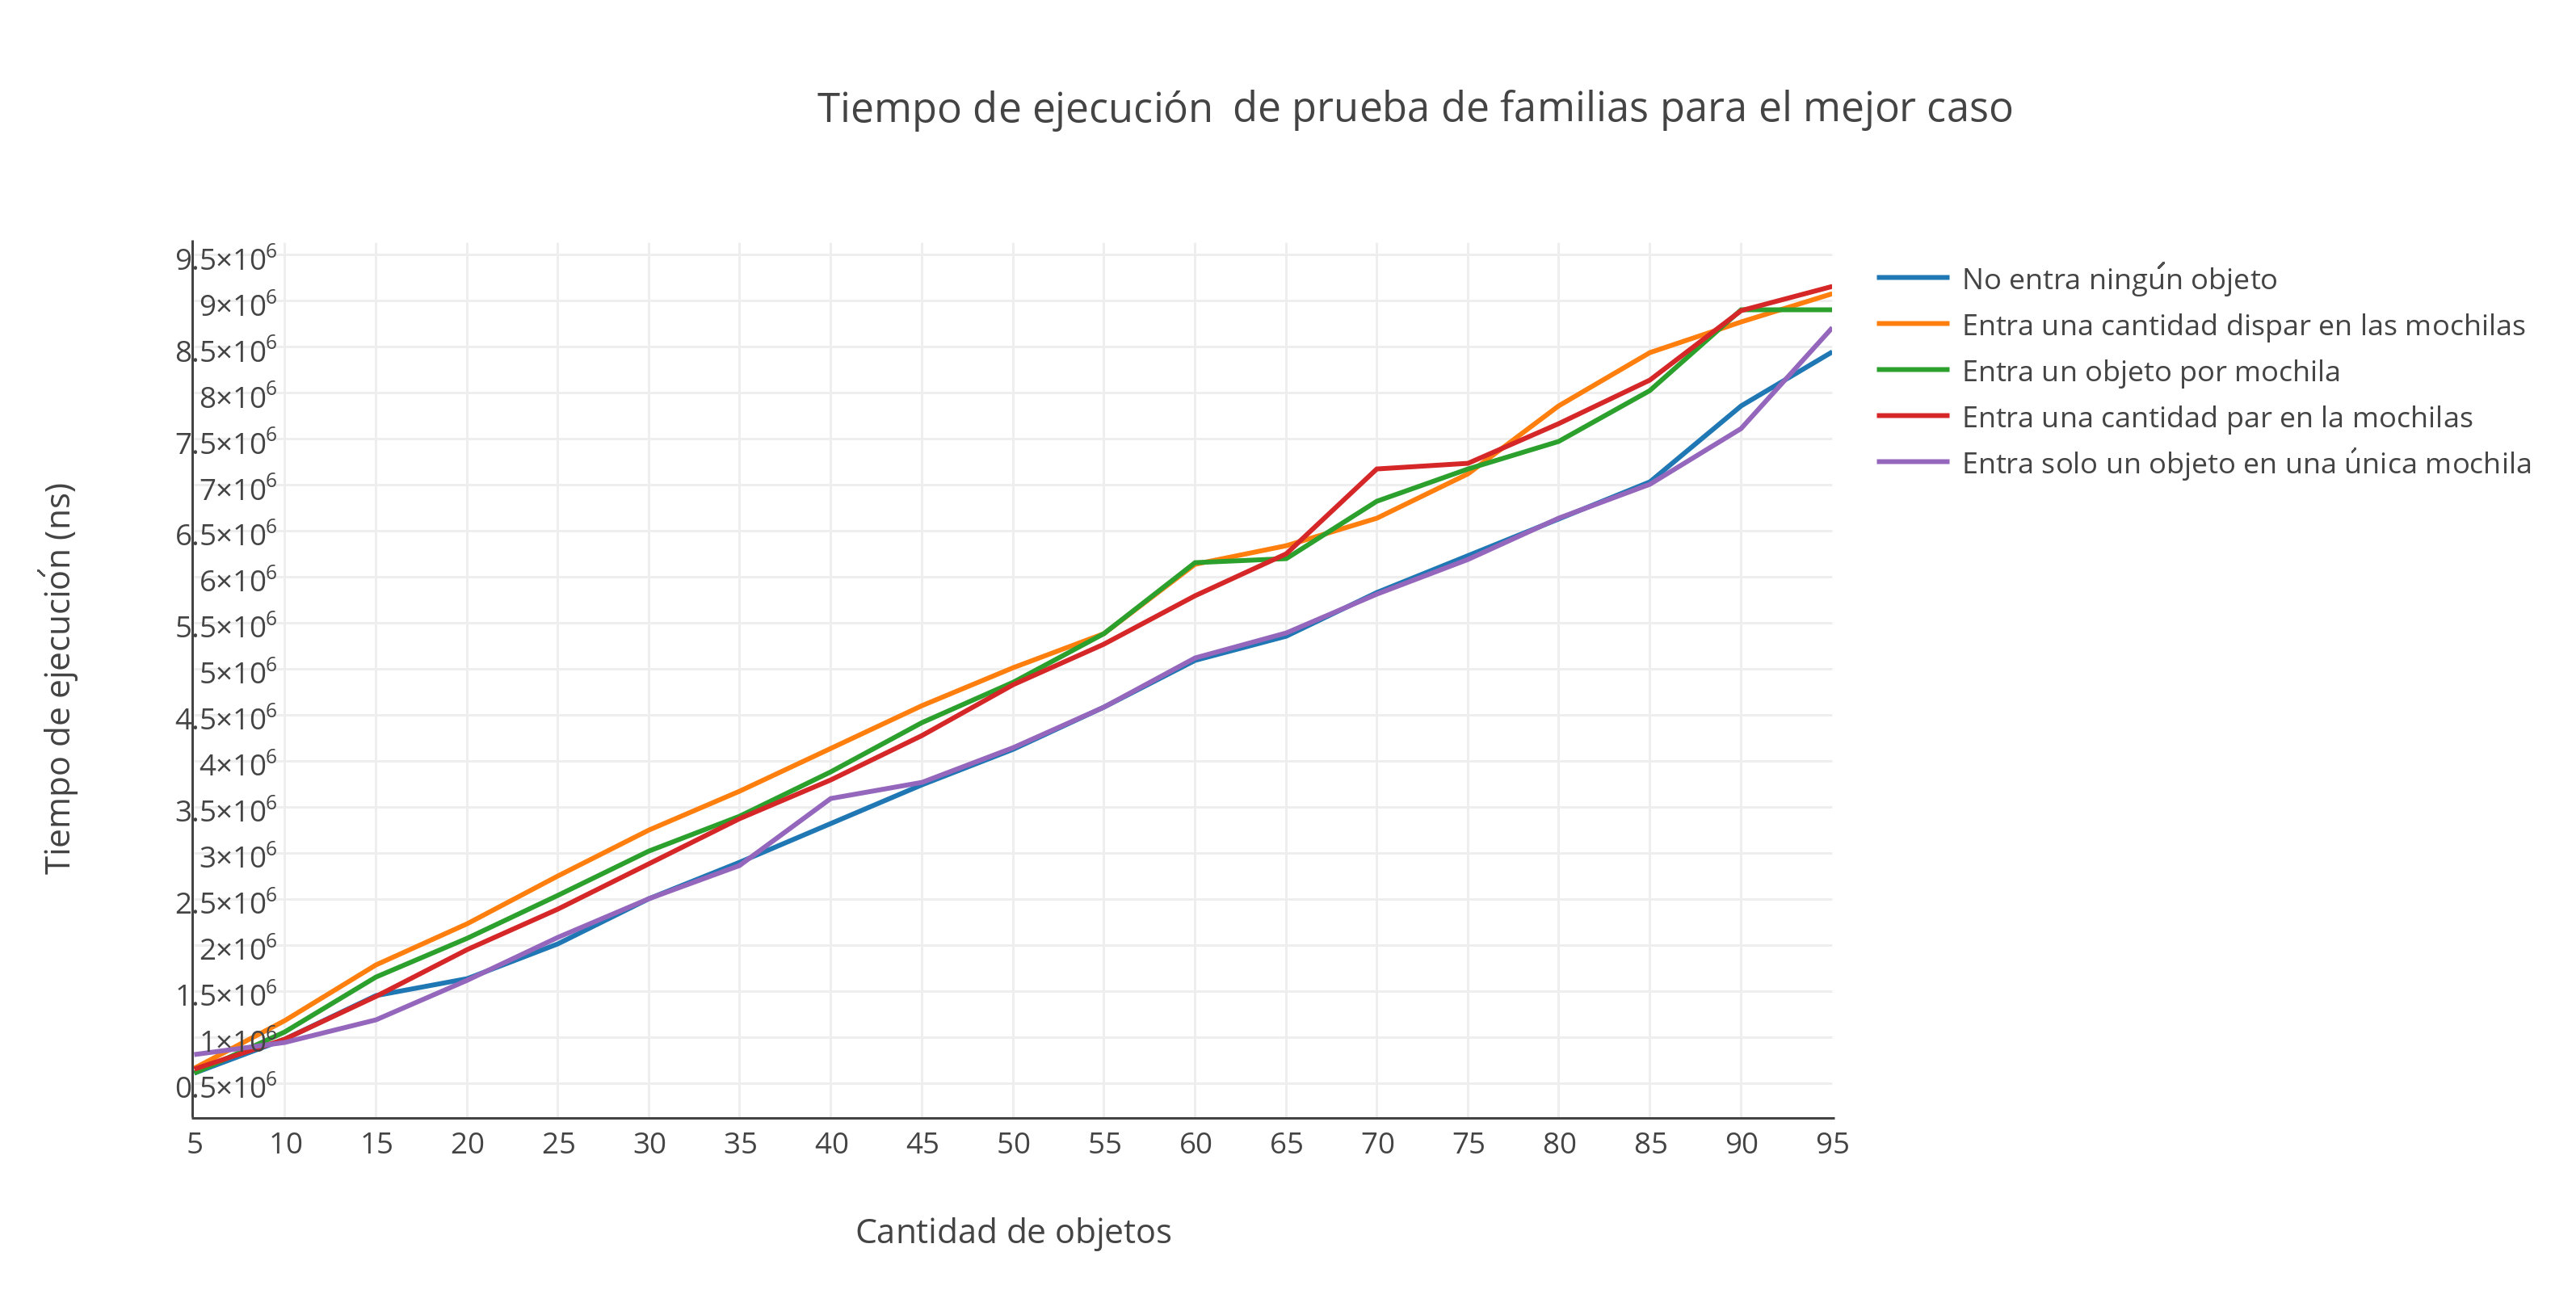
\includegraphics[scale=0.65]{./EJ3/comparativo1.png}
 {$Gr$\'a$fico$ \ 3.2 - $Comparativo$ $2$}
  \end{center}
  \vspace*{0.3cm}

Las familias de casos que fueron representadas en los gr\'aficos han sido las siguientes:\\
\begin{itemize}
\item No entra ning\'un objeto en las mochilas
\item Entra un \'unico objeto en cada mochila
\item Entra un \'unico objeto en total
\item Entra una cantidad par de objetos en cada mochila
\item Entra una cantidad dispar de objetos en cada mochila
\item Entran todos los objetos en las mochilas
\end{itemize}

Se puede observar en el gr\'afico 3.1 como la familia 6 de casos crece mucho m\'as r\'apido que el resto de las familias generando as\'i que en el gr\'afico 3.1 no se pueda distinguir de buena forma el resto de las 6 familias, es por esto que en el gr\'afico 3.2 solo fueron representadas estas 6.\\

Se puede observar entre el gr\'afico 3.1 y 3.2 en los cuales la familia \textbf{Entran todos los objetos en las mochilas} es el peor caso, debido a que nuestro algoritmo deber\'a chequear por cada objeto en que mochila colocarlo ya que tendr\'a la posibilidad de maximizar la totalidad colocando al objeto en alguna de las 3.\\

Luego, en el gr\'afico 3.2 se puede observar como tanto la familia de casos en las que no entra ning\'un objeto o entra unicamente uno se ven m\'as beneficiadas por la implentaci\'on de nuestro algoritmo el cual verificar\'a si es posible o no meter al objeto en cuesti\'on dentro de alguna de las mochilas, y como el peso del mismo es superior a la capacidad de las 3 mochilas directamente lo descarta sin tener que realizar el chequeo de maximizaci\'on.

Podemos concluir entonces que, el mejor caso para nuestro algoritmo es en el cual \textbf{No entra ning\'un objeto en las mochilas} ya que como mencionamos, nuestro algoritmo solo verificara su peso y al ser mayor descartara al objeto y no tendra que realizar los chequeos de maximizaci\'on.\\

A continuaci\'on mostraremos un gr\'afico que representa lo enunciado:

\vspace*{0.3cm} \vspace*{0.3cm}
  \begin{center}
 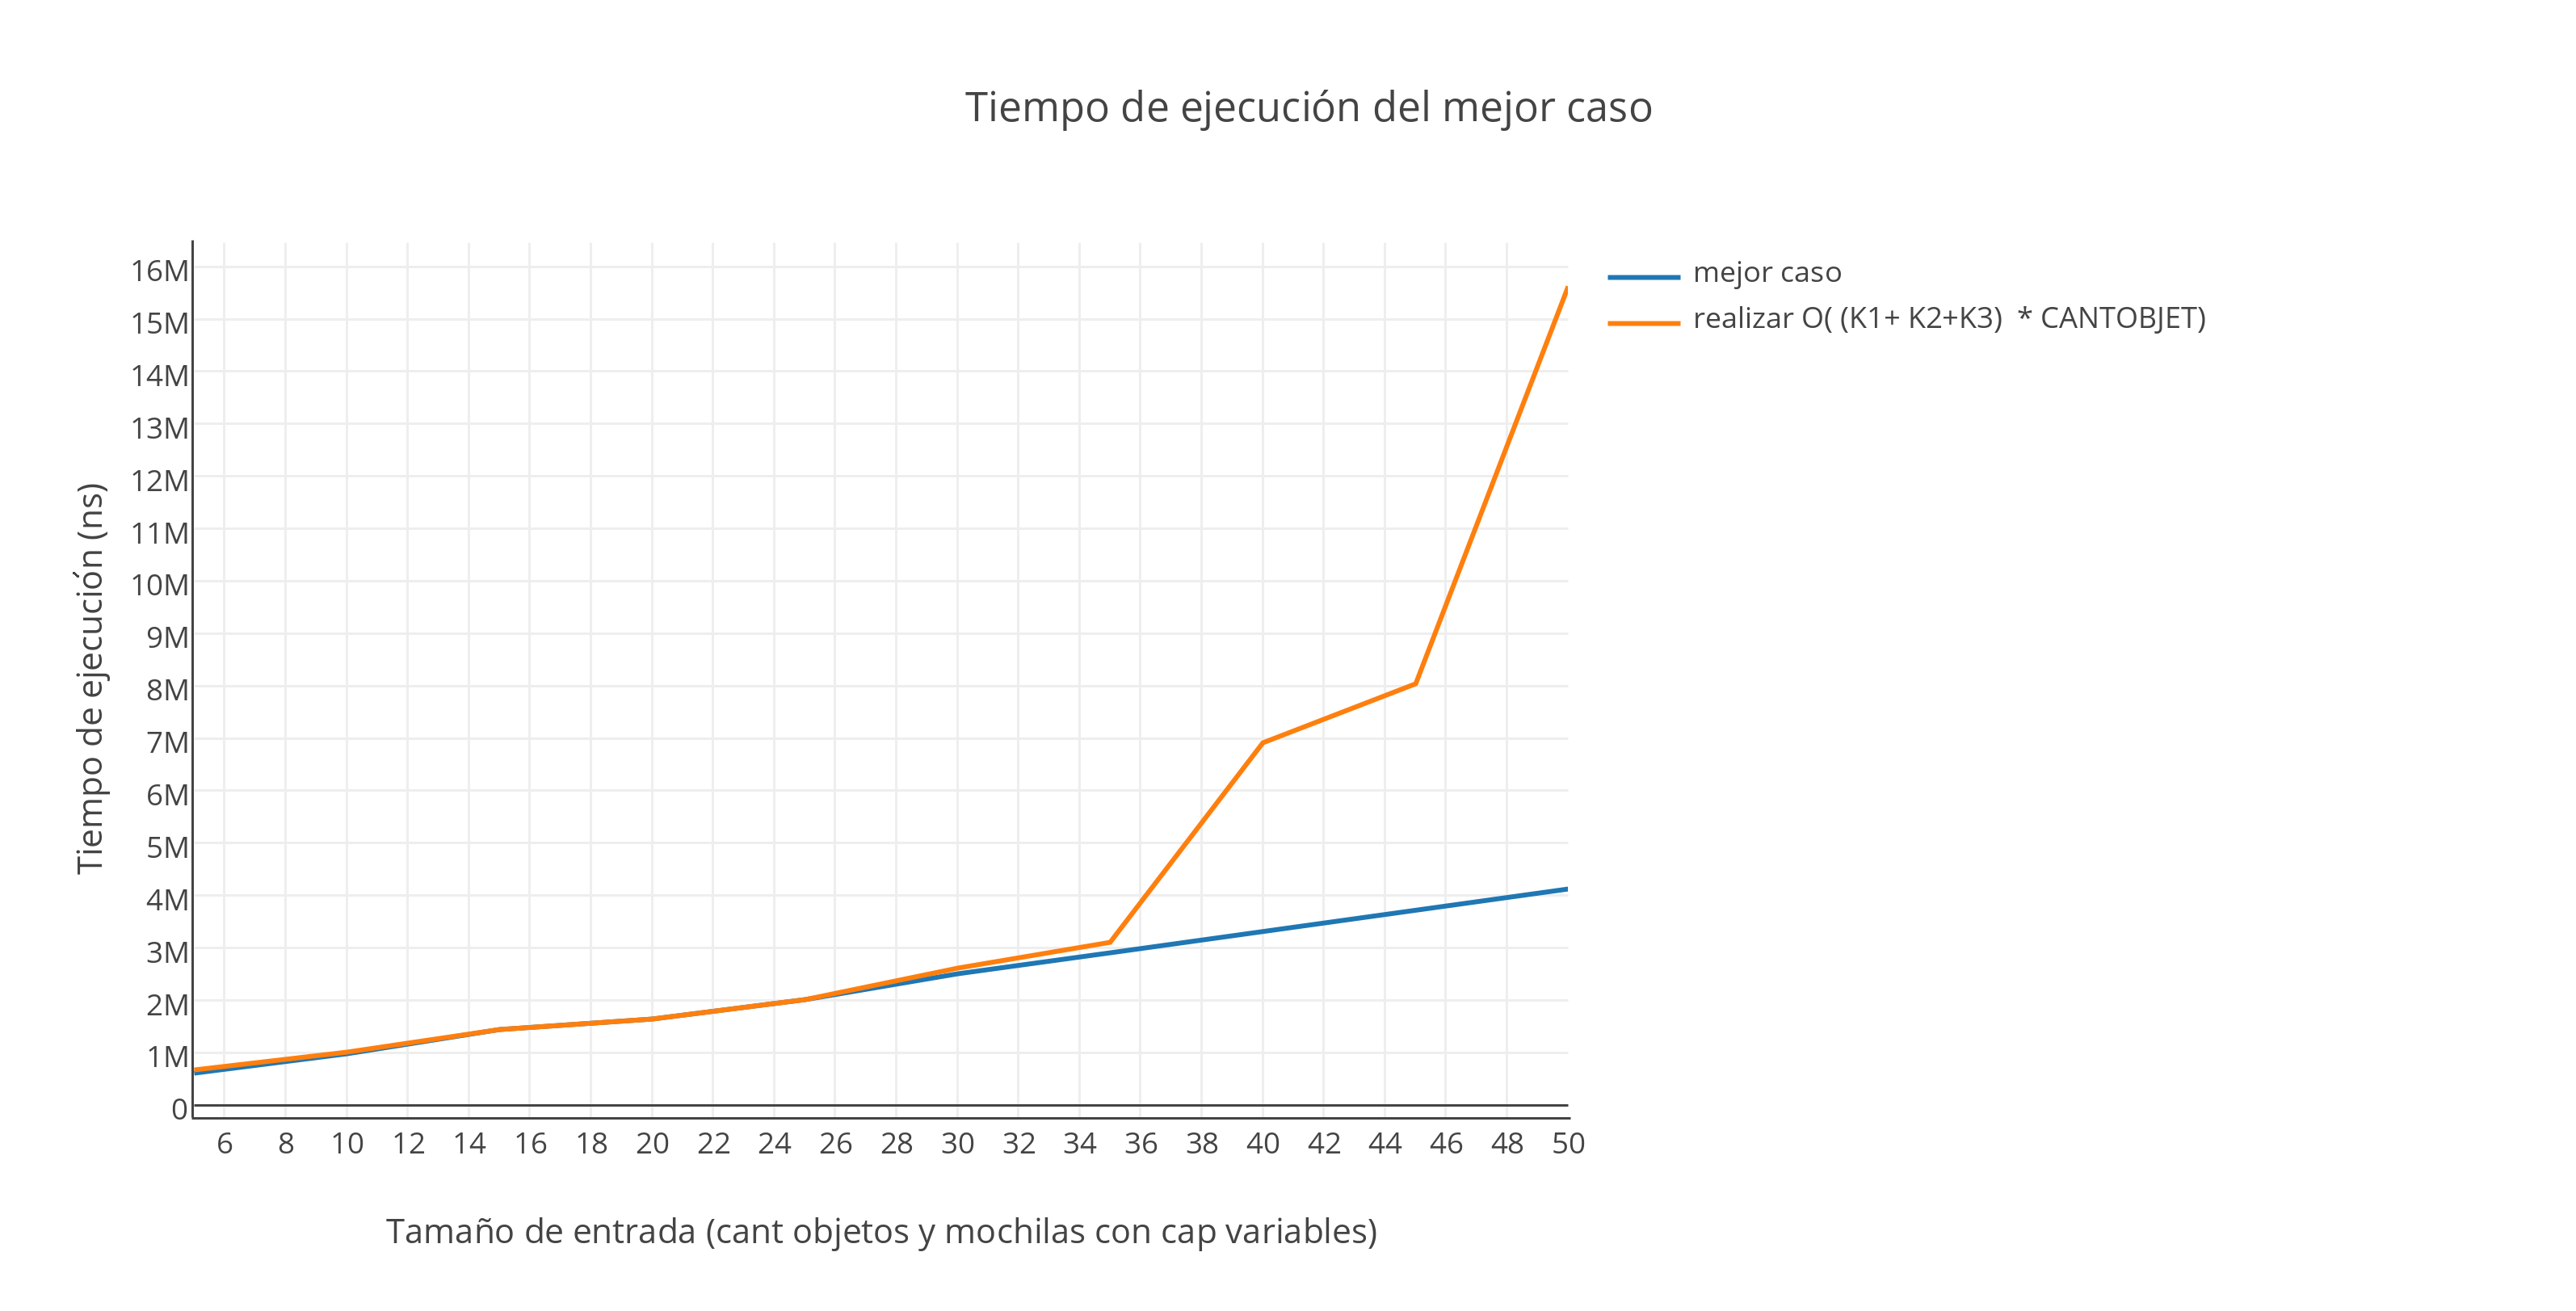
\includegraphics[scale=0.65]{./EJ3/mejorcaso.png}
 {$Gr$\'a$fico$ \ 3.3 - $Mejor$ $caso$ $del$ $algoritmo$}
  \end{center}
  \vspace*{0.3cm}

Dividiendo por la complejidad calculada se obtuvo lo siguiente:\\

\vspace*{0.3cm} \vspace*{0.3cm}
  \begin{center}
 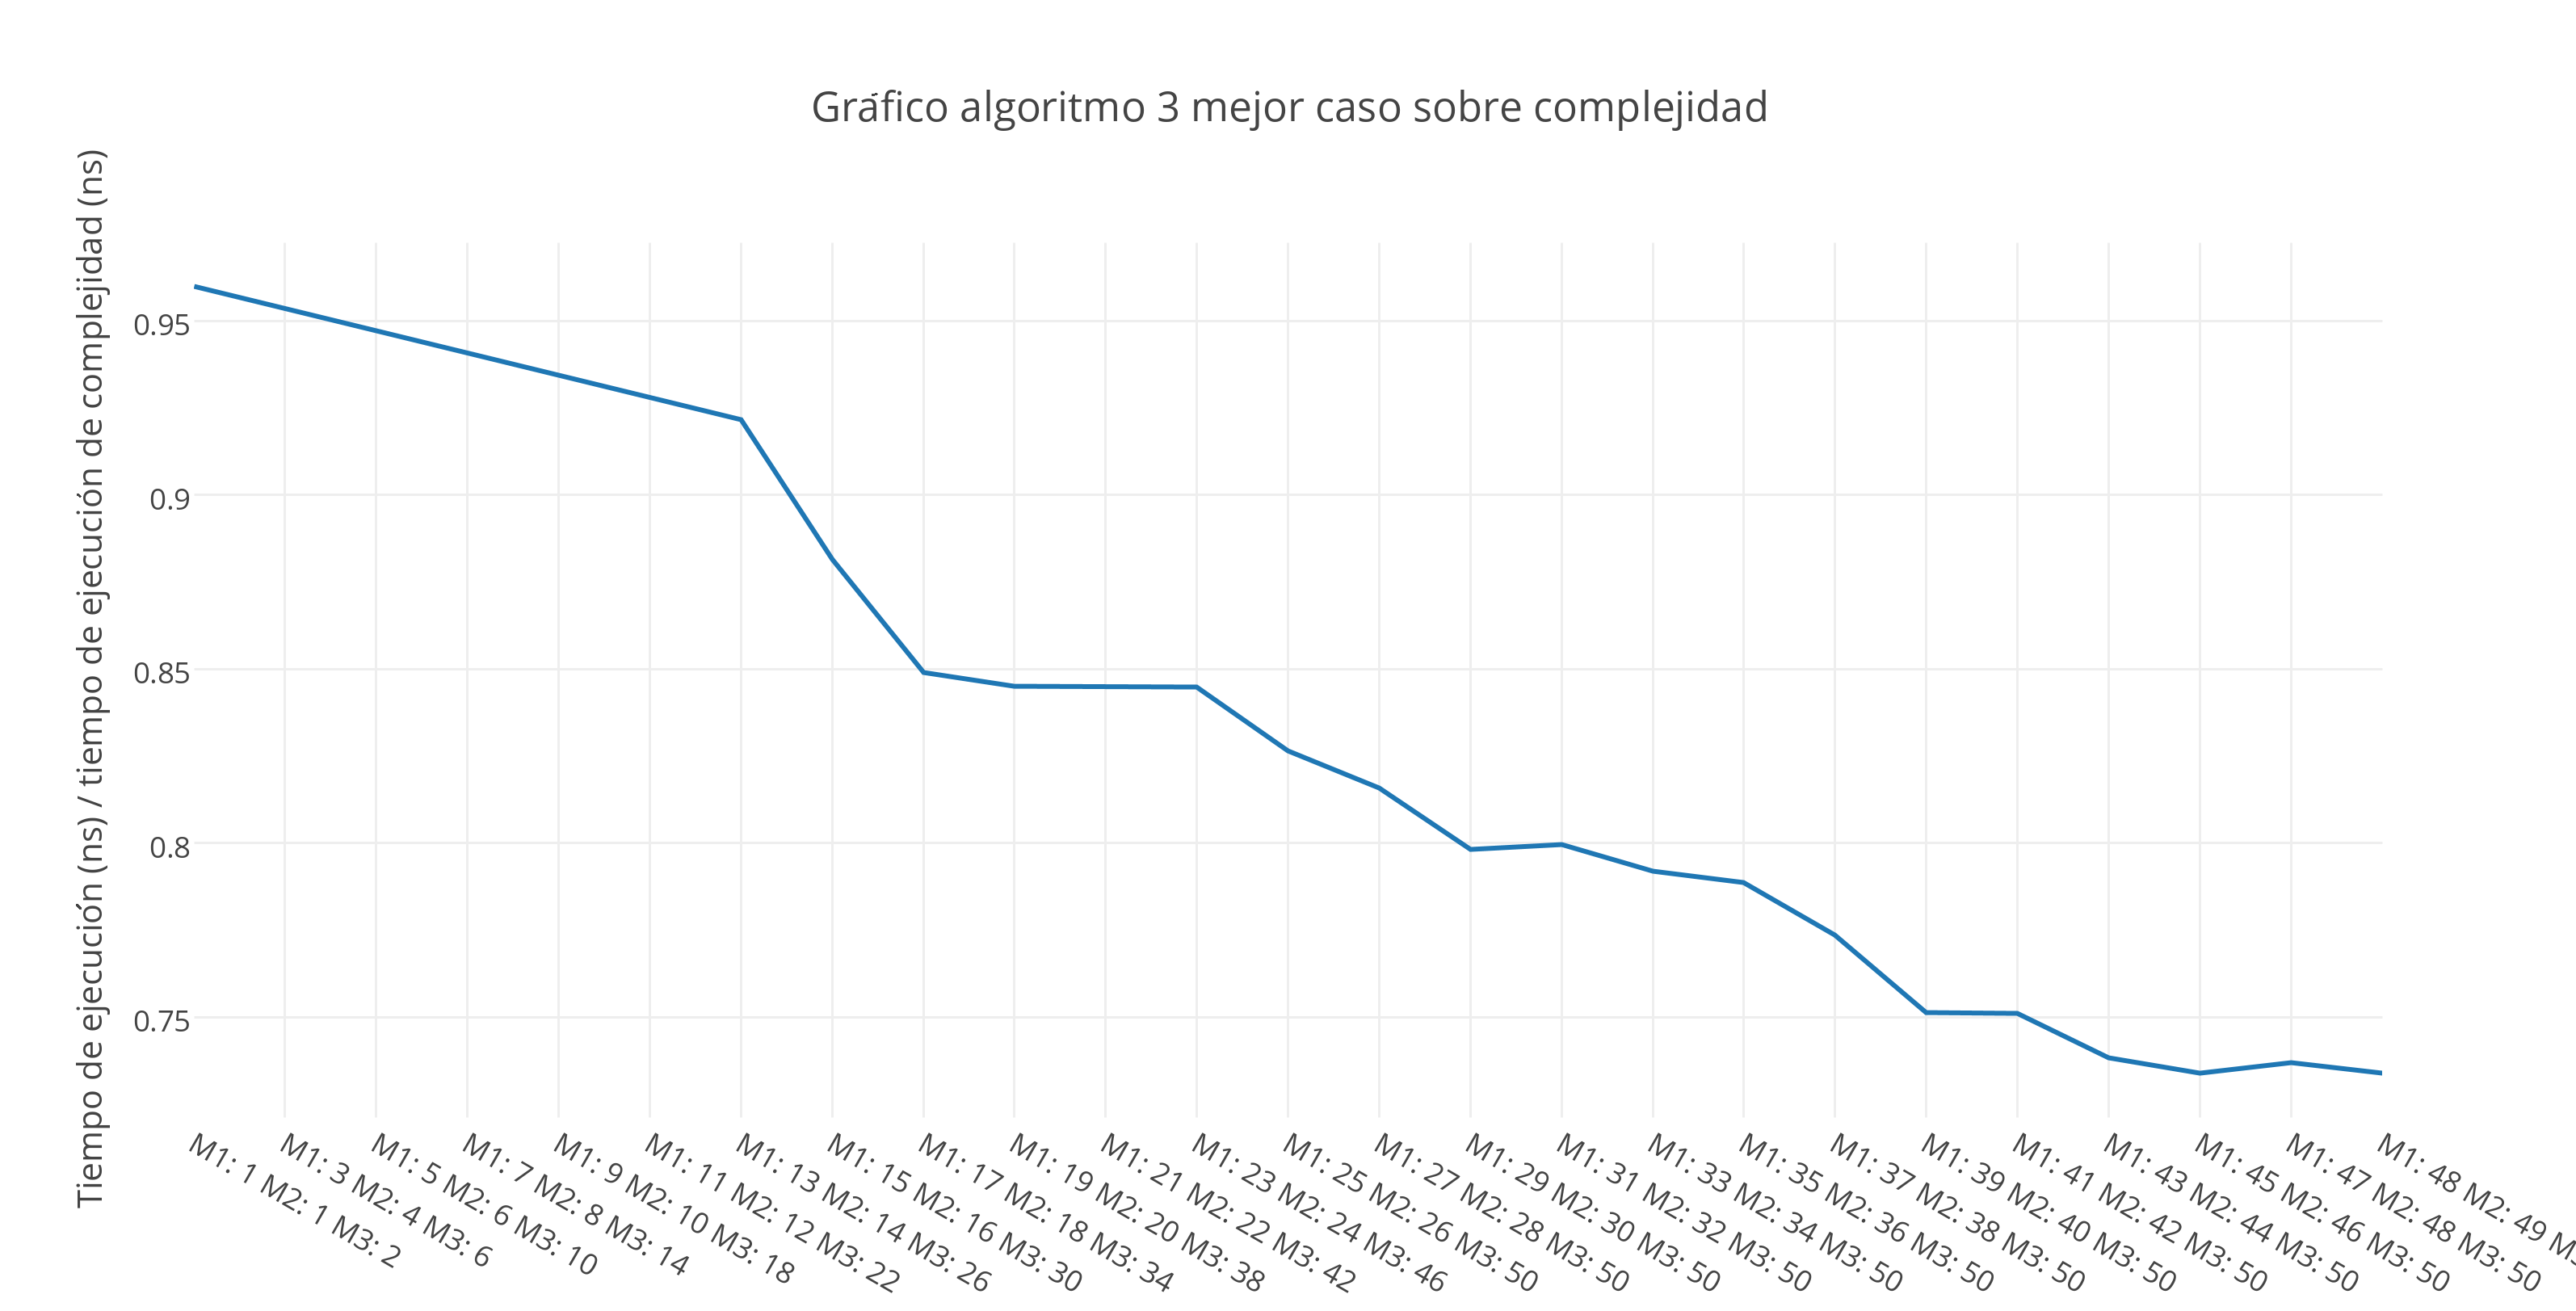
\includegraphics[scale=0.65]{./EJ3/mejorcaso1.png}
 {$Gr$\'a$fico$ \ 3.4 - $Mejor$ $caso$ $del$ $algoritmo$ $sobre$ $complejidad$}
  \end{center}
  \vspace*{0.3cm}
  
Se puede ver en el gr\'afico 3.3 que, nuestro algoritmo, esta acotado por la funci\'on de la cota te\'orica, ya que el mismo realizara una cantidad sustancialmente menor de chequeos e iteraciones por verificar inicialmente si los objetos tienen la posiblidad o no de ingresar en las mochilas.\\

Luego, en el gr\'afico 3.4, en el cual dividimos el tiempo de ejecuci\'on de dicho caso con el tiempo de realizar O(\[
\sum_{i=1}^{3}K_{i} 
\] $\ast CantObjetos$) operaciones nos da una funci\'on resultante la cual se encuentra por debajo de 1 y tiende a 0 cuando la entrada aumenta corroborando lo que enunciamos.\\

Manteniendo el mismo razonamiento, el peor caso para nuestro algoritmo se da cuando \textbf{Entran todos los objetos en las mochilas} ya que el algoritmo deber\'a decidir en que mochila colocar el objeto para que el resultado sea \'optimo. Por consiguiente, mostraremos un gr\'afico que representa lo hablado:\\

\vspace*{0.3cm} \vspace*{0.3cm}
  \begin{center}
 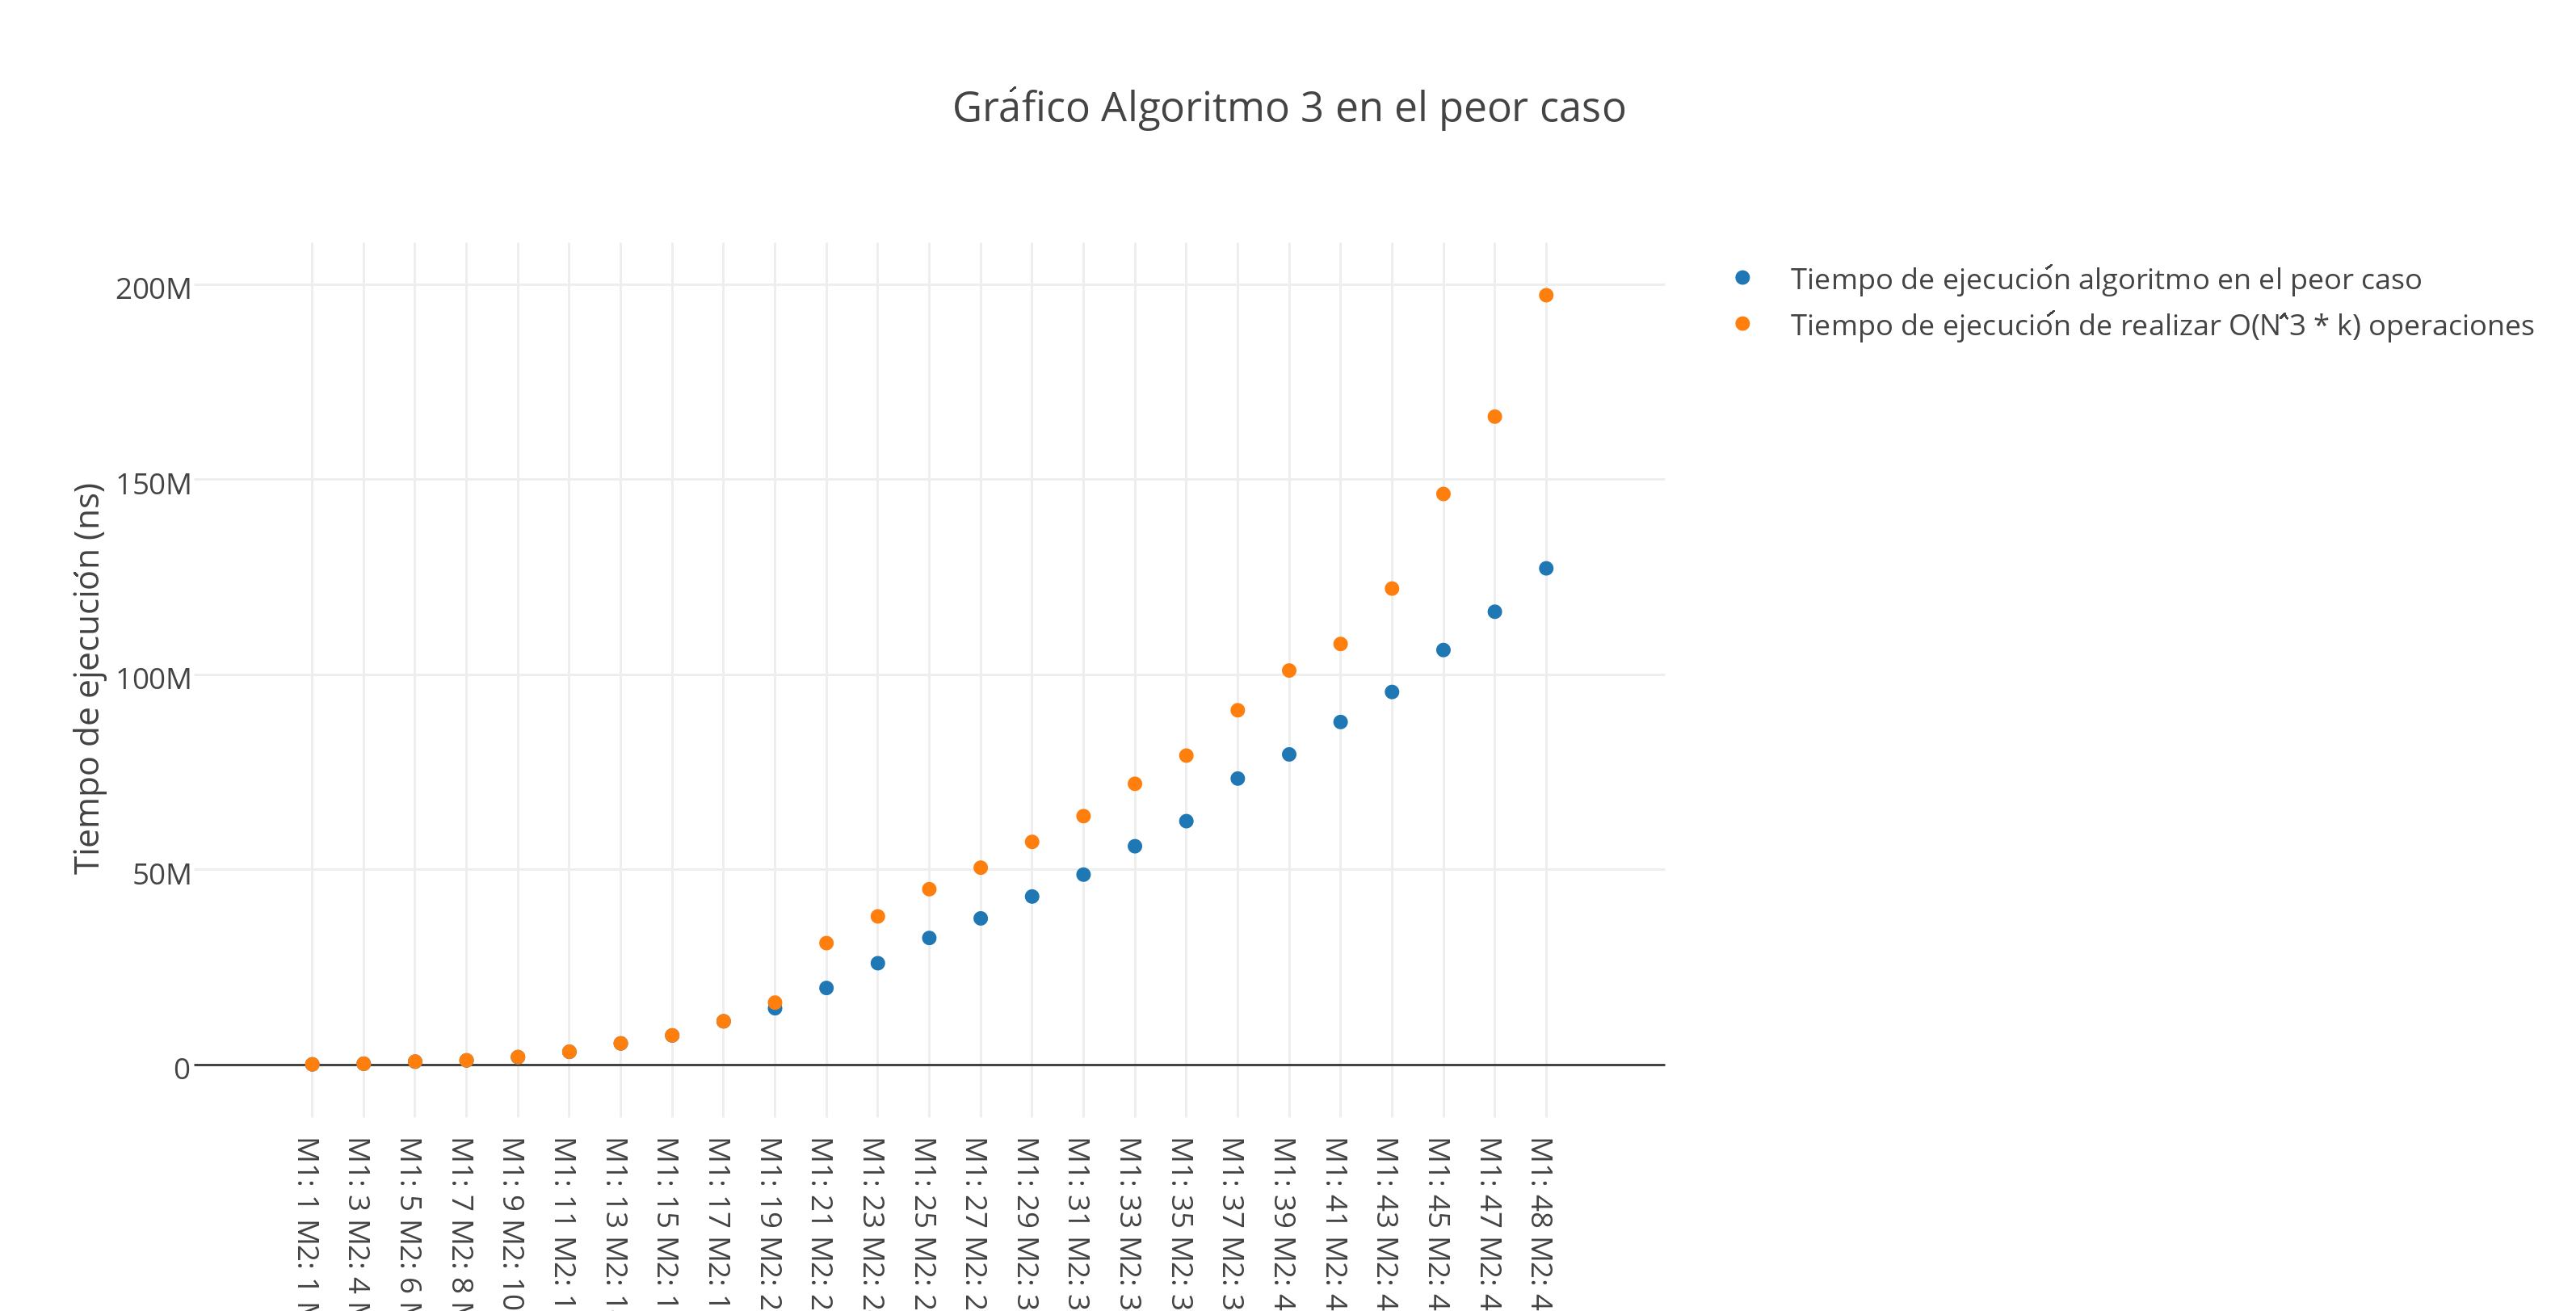
\includegraphics[scale=0.65]{./EJ3/peorcaso.png}
 {$Gr$\'a$fico$ \ 3.5 - $Peor$ $caso$ $del$ $algoritmo$}
  \end{center}
  \vspace*{0.3cm}

Dividiendo por la complejidad calculada se obtuvo lo siguiente:\\

\vspace*{0.3cm} \vspace*{0.3cm}
  \begin{center}
 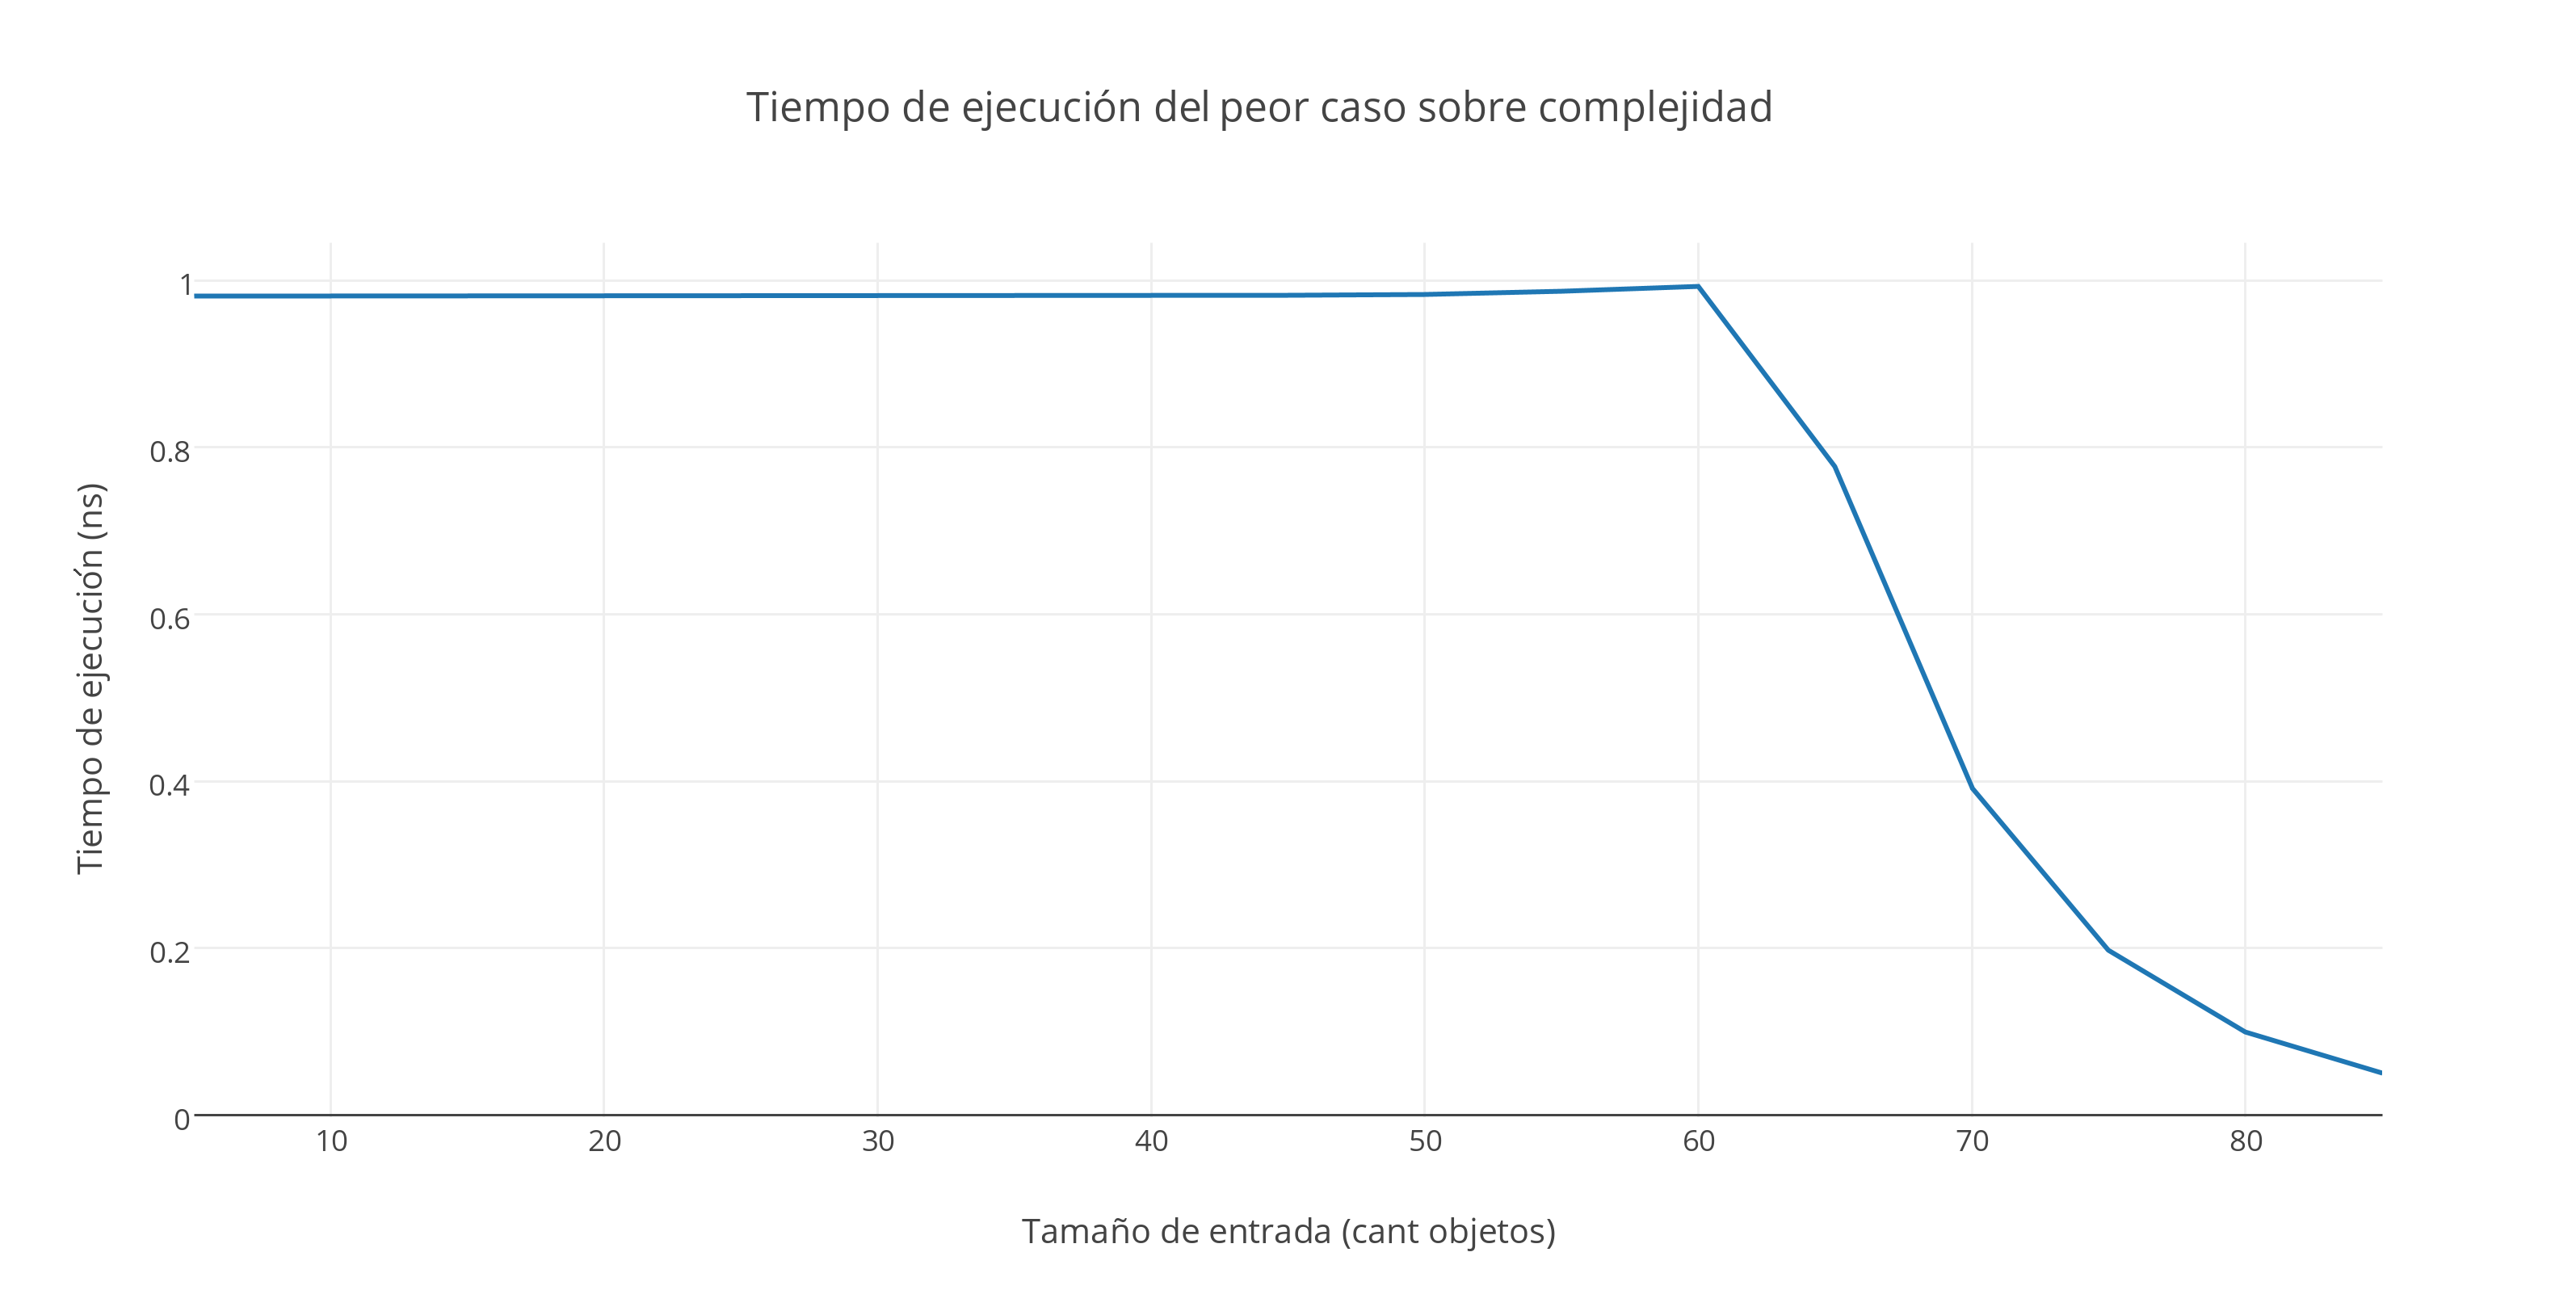
\includegraphics[scale=0.65]{./EJ3/peorcaso1.png}
 {$Gr$\'a$fico$ \ 3.6 - $Peor$ $caso$ $del$ $algoritmo$ $sobre$ $complejidad$}
  \end{center}
  \vspace*{0.3cm}
  
  
Es posible observar en el gr\'afico 3.4 que, dado nuestro algoritmo, al tener las pobilidad de ir metiendo cada uno de los objetos en las mochilas, el mismo realizar\'a la optimizaci\'on de 3 matrices que simbolizan a cada mochila anidadas, lo que nos dar\'a una complejidad acotada por la capacidad de las mochilas por la cantidad de elementos que en esta evaluaci\'on es constante, simplificando lo dicho nos quedar\'ia O(\[
\sum_{i=1}^{3}K_{i} 
\] $\ast CantObjetos$) .\\
Luego, en el gr\'afico 3.4, en el cual dividimos el tiempo de ejecuci\'on de dicho caso con el tiempo de realizar O(\[
\sum_{i=1}^{3}K_{i} 
\] $\ast CantObjetos$) operaciones nos devuelve una funci\'on resultante la cual se encuentra por debajo de 1 y tiende a 0 cuando la entrada aumenta corroborando lo que acabamos de decir.\\

Por \'ultimo un grafico comparativo entre el mejor y peor caso y la cota teorica nos otorga la siguiente percepci\'on:\\ 

\vspace*{0.3cm} \vspace*{0.3cm}
  \begin{center}
 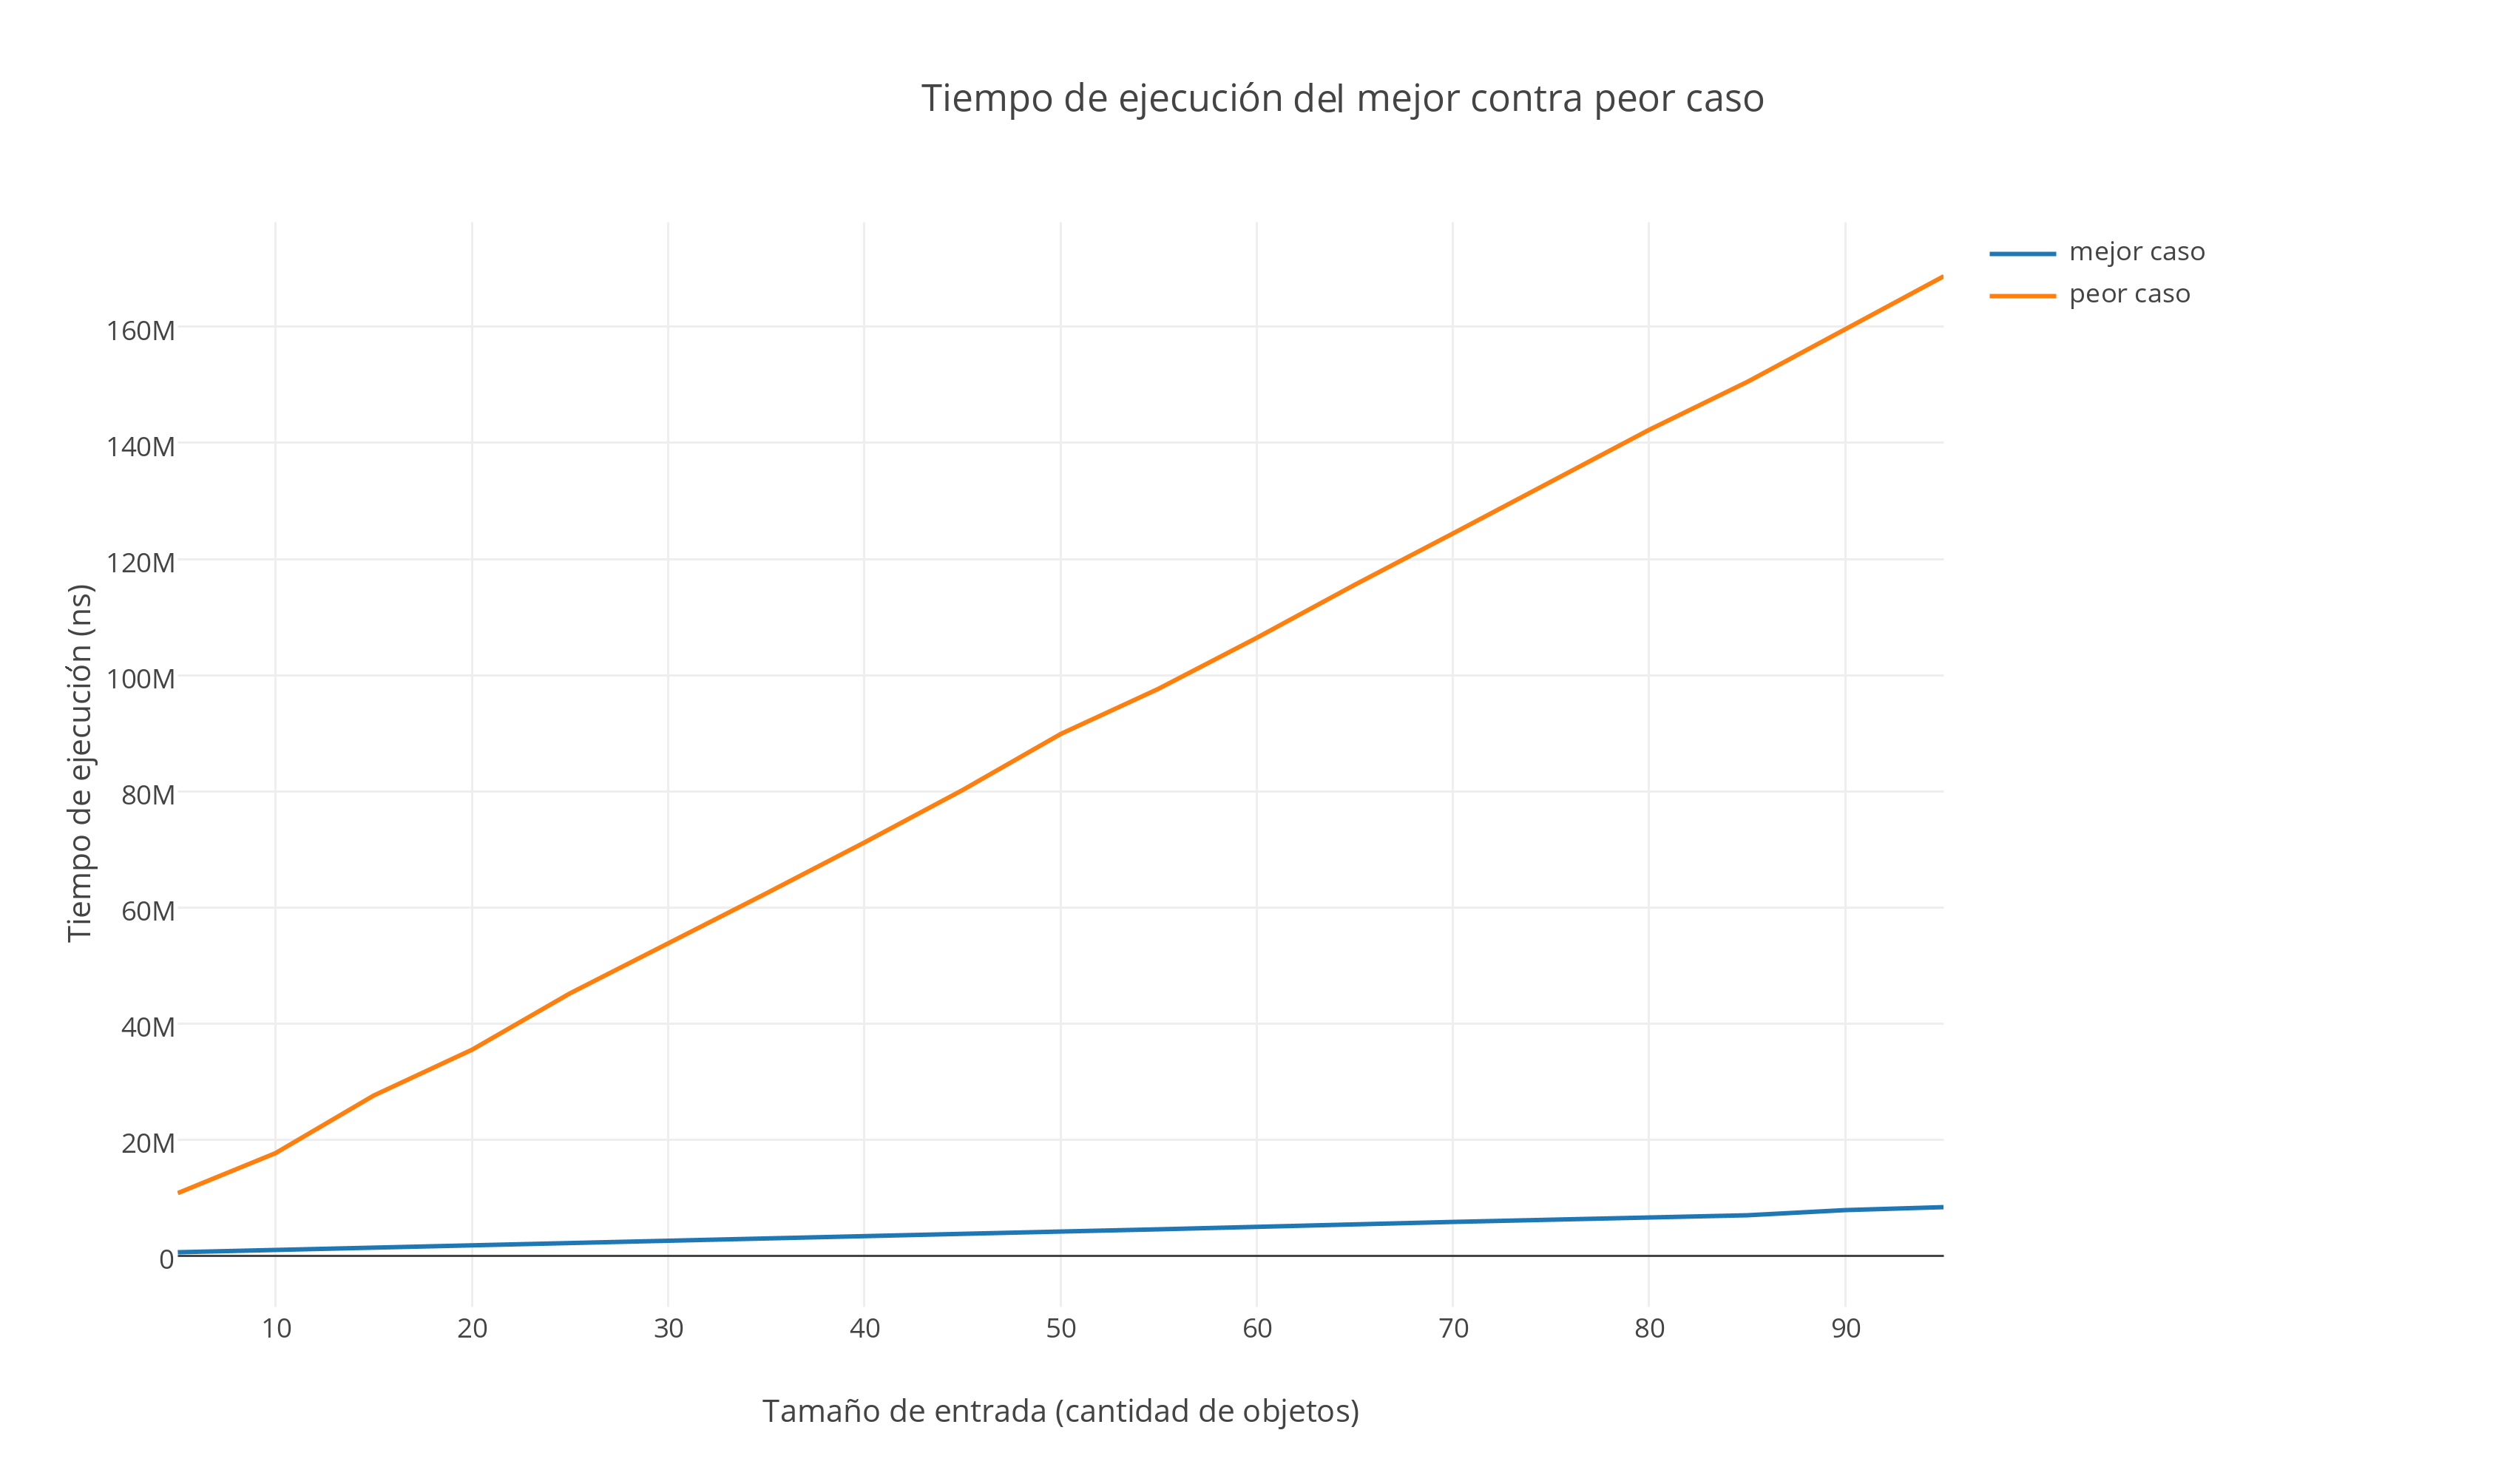
\includegraphics[scale=0.65]{./EJ3/comparativo2.png}
 {$Gr$\'a$fico$ \ 3.7 - $Comparativo$ $peor$ $y$ $mejor$ $caso$ $del$ $algoritmo$}
  \end{center}
  \vspace*{0.3cm}


\vspace*{0.3cm} \vspace*{0.3cm}
  \begin{center}
 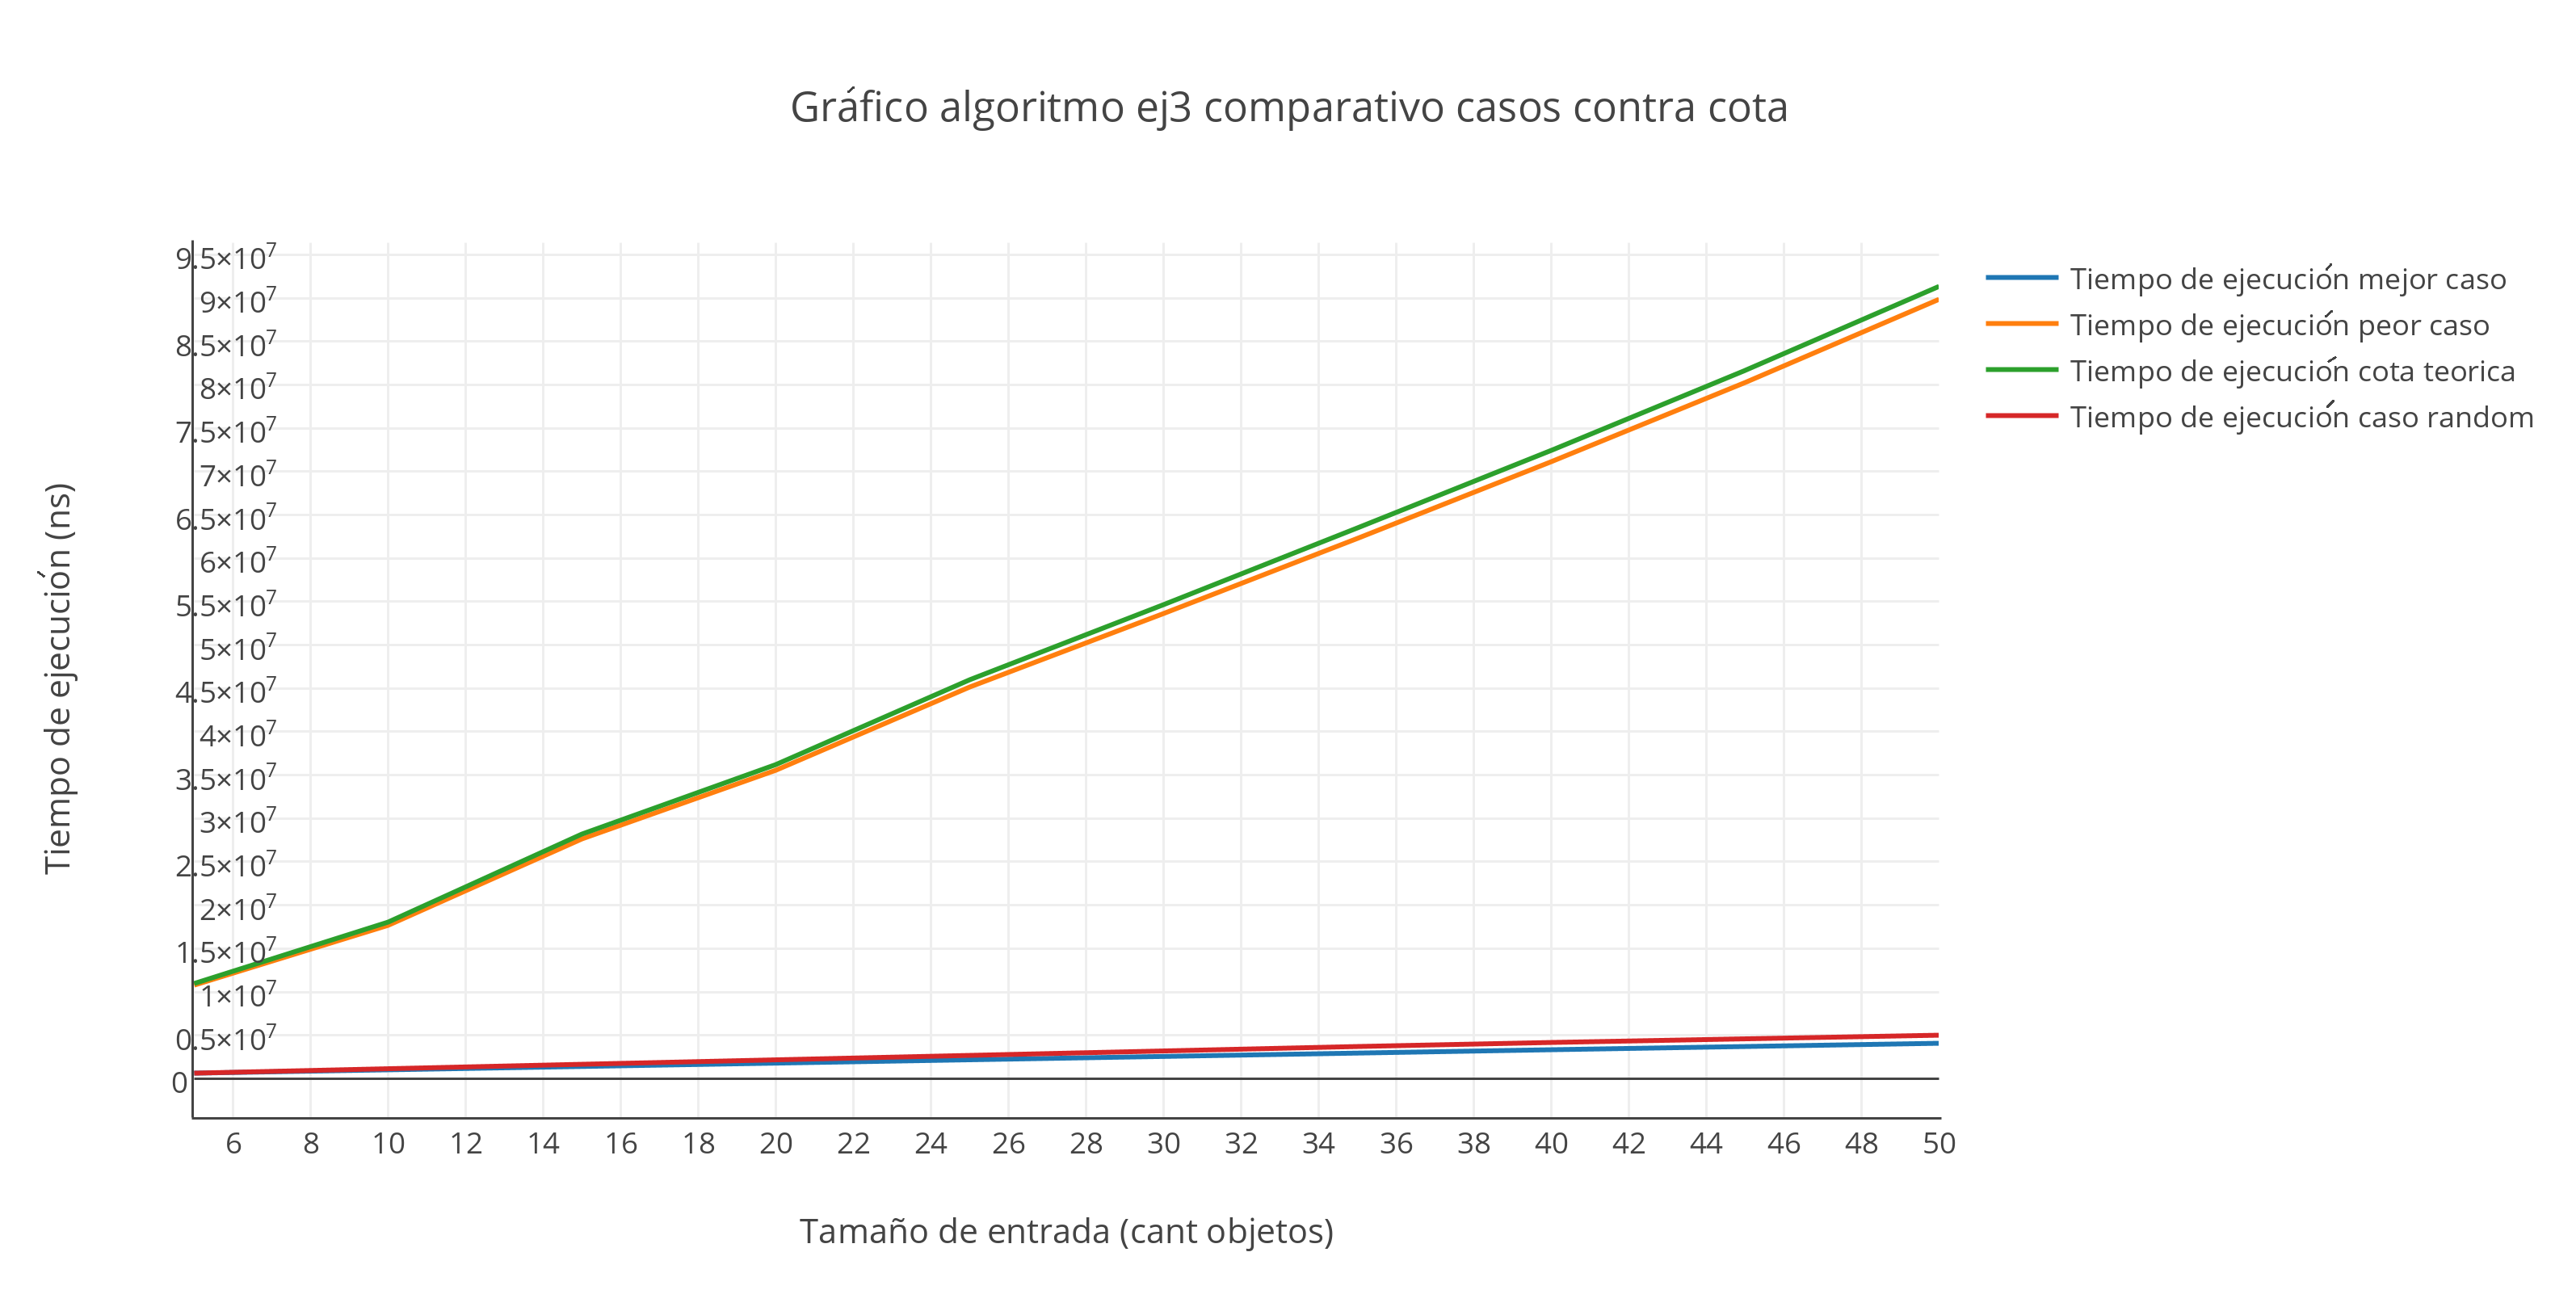
\includegraphics[scale=0.65]{./EJ3/comparativo3.png}
 {$Gr$\'a$fico$ \ 3.8 - $Comparativo$ $peor$ $y$ $mejor$ $caso$ $del$ $algoritmo$ $contra$ $complejidad$ $te\'orica$}
  \end{center}
  \vspace*{0.3cm}

Es notorio que, en el gr\'afico 3.8 la funciones resultantes siempre se mantienen por debajo de la cota de complejidad calculada anteriormente, con lo cual se ve que tanto en el mejor como en el peor caso nuestro algoritmo sigue estando acotado por la misma.\\
